\chapter{Implementación}
Durante la implementación, se ha seguido la planificación y metodologías
anteriormente descritas, dividiendo el proyecto en tareas más pequeñas y
manejables, para que se puedan realizar en un periodo de tiempo razonable.

Al emplearse la metodología \textit{Scrum}, se realizan primero las tareas más
prioritarias, como la creación de la infraestructura y la ingesta de las fuentes
esenciales, y se dejan para más adelante tareas como la visualización para
clientes externos o fuentes menos críticas y más complejas, como las APIs de
terceros o el \textit{web scraping}.

Con el objetivo de realizar un desarrollo iterativo y ágil, se desarrolla
primero de todo un prototipo de despliegue en local, para posteriormente
migrar este despliegue a la nube. A continuación, se desarrollan los scripts de
ingesta de datos y se finaliza con la visualización de los datos en Kibana.

El burndown chart de la figura \ref{fig:burndown} muestra la evolución de las
tareas a lo largo del tiempo, y se puede observar cómo se han ido completando
las tareas planificadas.

\begin{figure}[htbp]
	\centering
	\begin{tikzpicture}
		\begin{axis}[
			title={Diagrama burndown del proyecto},
			date coordinates in=x,
			xmin={2024-03-18},
			xmax={2024-07-18},
			xtick={2024-03-18,2024-04-18,2024-05-18,2024-06-18,2024-07-18},
			xticklabel style={rotate=45,anchor=east},
			xticklabel={\day-\month},
			ylabel={Puntos de estimación restantes},
			ymin=0,
			ymax=41,
			grid=both,
			legend pos=north east,
			width=0.8\textwidth,
			height=0.6\textwidth,
		]
			% Línea ideal
			\addplot[blue] coordinates {
				(2024-03-18,41)
				(2024-07-18,0)
			};

			% Línea MVP
			\addplot[blue,dashed] coordinates {
				(2024-03-18,41)
				(2024-07-18,11)
			};

			% Progreso real
			\addplot[red,mark=*] coordinates {
				(2024-03-18,41)
				(2024-04-18,36)
				(2024-05-18,28)
				(2024-06-18,17)
				(2024-07-18,10)
			};

			\legend{Ideal,MVP,Real}
		\end{axis}
	\end{tikzpicture}
	\caption{Diagrama Burndown que representa el progreso del proyecto}
	\label{fig:burndown}
\end{figure}

La estimación de las tareas se realizó en el apartado \fullref{sec:planif_inicial}.

\newpage{}
La línea azul representa el progreso ideal, mientras que la línea roja muestra
el progreso real. Se toma el 18 de marzo como fecha de inicio del proyecto y el
18 de julio como fecha de finalización. Se puede observar cómo el progreso real
sigue la línea ideal, aunque con algunas desviaciones debido a la naturaleza
iterativa del desarrollo.

Pese a que el progreso del desarrollo no ha sido completamente óptimo, se ha
logrado superar los objetivos principales del proyecto, entregando un producto
mínimo viable (MVP) de calidad y sentando las bases para futuras iteraciones.

\newpage{}
\section{Despliegue local}\label{sec:impl_local}
Para arrancar el desarrollo del proyecto, se implementa una versión local del
sistema, que permita trabajar en un entorno controlado y sin dependencias
externas para comprobar su correcto funcionamiento y establecer
las configuración base para su posterior despliegue en la nube.

Puesto que se ha decidido utilizar Docker para la gestión de contenedores, se
crea un archivo \texttt{docker-compose.yml} que define los servicios
necesarios para el proyecto, es decir, \textit{Kafka}, \textit{Zookeeper},
\textit{Elasticsearch}, \textit{Kibana} y \textit{Logstash}, ignorando por
el momento la ingesta de datos y la escalabilidad del sistema.

Para la configuración de los servicios, se ha creado un archivo \texttt{.env}
que define las variables de entorno necesarias para el correcto funcionamiento
de los servicios, como las contraseñas o la versión del \textit{stack}.

Esta sección de la documentación documenta el desarrollo de la historia de
usuario inicial, de acuerdo con lo establecido en la sección \fullref{sec:planif_inicial}:

\begin{table}[H]
	\centering
	\begin{tabular}{|p{0.7\linewidth}|c|c|}
		\hline
		\textbf{Nombre} & \textbf{Prioridad} & \textbf{Tamaño} \\
		\hline
		\hline
		Creación de la infraestructura base (técnica) & P0\cellcolor{red!50} & L\cellcolor{orange!50} \\
		\hline
  	\end{tabular}
  	\caption{Lista de HUs cumplimentadas con el despliegue local}
  	\label{tab:impl_local}
\end{table}


\newpage{}
\subsection{Explicación del código}
\emph{El código de despliegue local se encuentra en el anexo \fullref{anexo:local}.}

A nivel de configuración, se definen variables de entorno para cada contenedor
mediante el uso de la palabra clave \texttt{environment} y las claves definidas
por cada imagen. Para cada contenedor, se define además información adicional
dependiendo de las características del servicio, como la dependencia en otras
imágenes, los límites de recursos o los puertos de escucha.

Para evitar el ruido excesivo por consola una vez arrancado los servicios, se
reduce el nivel de \textit{logging} a \textit{WARN} en los servicios que lo
soporten.

Durante el arranque de los contenedores, se ejecuta un script de inicialización
que se encarga de crear las credenciales y los usuarios necesarios para el
funcionamiento de los servicios. Estas credenciales son necesarias ya que los
contenedores funcionan mediante tráfico HTTPS.

Los contenedores cuentan con comprobaciones de salud (o \textit{health-checks})
básicas para asegurar que los servicios se han arrancado correctamente y están
funcionando. Los \textit{health-checks} son normalmente comprobaciones de
disponibilidad de un servicio, como la respuesta de un puerto o la existencia de
un archivo.

Al comienzo del archivo \texttt{docker-compose.yml}, se definen los volúmenes y
las redes necesarias para el correcto funcionamiento de los servicios.

\begin{lstlisting}[style=yaml, caption={Definición de volúmenes y redes en Docker Compose}]
volumes:
	es01data:
	kibanadata:
	elasticdata:
	logstashdata:
	kafkadata:
	certs:

networks:
	default:
		driver: bridge
\end{lstlisting}

A continuación, se definen los servicios necesarios para el proyecto, comenzando
por el contenedor de preparación de credenciales y usuarios. Se utiliza una
imagen de Elasticsearch para la creación de las credenciales, y se monta un
volumen para la persistencia de las mismas.

\begin{lstlisting}[style=yaml, caption={Definición del servicio de preparación}]
setup:
  image: docker.elastic.co/elasticsearch/elasticsearch:${STACK_VERSION}
  volumes:
    - certs:/usr/share/elasticsearch/config/certs
    - ./setup.sh:/usr/local/bin/setup.sh
  user: root
  container_name: setup
  command: ["/bin/bash", "/usr/local/bin/setup.sh"]
  healthcheck:
    test: [ "CMD-SHELL", "[ -f config/certs/es01/es01.crt ]" ]
    interval: 5s
    timeout: 10s
    retries: 10
\end{lstlisting}

El servicio de preparación necesita tener una comprobación de salud, puesto que
el resto de contenedores lo tienen marcado como dependencia para su arranque. En
este caso, la comprobación consiste en la existencia de un archivo de
certificado.

Una vez definido el servicio de preparación, se definen los servicios de
\textit{Kafka} y \textit{Zookeeper}, que se basan en imágenes oficiales de
\textit{Confluent}.

\begin{lstlisting}[style=yaml, caption={Definición de los servicios de Kafka}]
zookeeper:
	container_name: zookeeper
	image: confluentinc/cp-zookeeper:latest
	environment:
	ZOOKEEPER_CLIENT_PORT: 2181
	ZOOKEEPER_TICK_TIME: 2000
	ZOO_LOG4J_PROP: WARN,CONSOLE
	ports:
	- 2181:2181

kafka:
	container_name: kafka
	image: confluentinc/cp-kafka:latest
	depends_on:
		- zookeeper
		- es01
	ports:
		- 9092:9092
		- 29092:29092
	environment:
		KAFKA_BROKER_ID: 1
		KAFKA_ZOOKEEPER_CONNECT: zookeeper:2181
		KAFKA_ADVERTISED_LISTENERS: LISTENER_DOCKER_INTERNAL://kafka:29092,LISTENER_DOCKER_EXTERNAL://localhost:9092
		KAFKA_LISTENER_SECURITY_PROTOCOL_MAP: LISTENER_DOCKER_INTERNAL:PLAINTEXT,LISTENER_DOCKER_EXTERNAL:PLAINTEXT
		KAFKA_INTER_BROKER_LISTENER_NAME: LISTENER_DOCKER_INTERNAL
		KAFKA_OFFSETS_TOPIC_REPLICATION_FACTOR: 1
		KAFKA_LOG4J_ROOT_LOGLEVEL: WARN
		KAFKA_TOOLS_LOG4J_LOGLEVEL: ERROR
		KAFKA_LOG4J_LOGGERS: 'kafka=WARN,kafka.controller=WARN,kafka.log.LogCleaner=WARN,state.change.logger=WARN,kafka.producer.async.DefaultEventHandler=WARN'
\end{lstlisting}

Ambos servicios cuentan con una serie de variables de entorno que definen su
configuración, como el puerto de escucha, el \textit{broker ID} o la dirección
de \textit{Zookeeper}.

Una vez definidos los servicios de Kafka, se define el servicio más crítico, el
contenedor de Elasticsearch, del que depende el funcionamiento de todo el
sistema.

\begin{lstlisting}[style=yaml, caption={Definición del servicio de Elasticsearch}]
es01:
    image: docker.elastic.co/elasticsearch/elasticsearch:${STACK_VERSION}
    container_name: es01
    restart: unless-stopped
    depends_on:
      - setup
    environment:
      - node.name=es01
      - cluster.name=${CLUSTER_NAME}
      - discovery.type=single-node
      - bootstrap.memory_lock=true
      - logger.level=WARN
      - ELASTIC_PASSWORD=${ELASTIC_PASSWORD}
      - xpack.security.enabled=true
      - xpack.security.http.ssl.enabled=true
      - xpack.security.http.ssl.key=certs/es01/es01.key
      - xpack.security.http.ssl.certificate=certs/es01/es01.crt
      - xpack.security.http.ssl.certificate_authorities=certs/ca/ca.crt
      - xpack.security.transport.ssl.enabled=true
      - xpack.security.transport.ssl.key=certs/es01/es01.key
      - xpack.security.transport.ssl.certificate=certs/es01/es01.crt
      - xpack.security.transport.ssl.certificate_authorities=certs/ca/ca.crt
      - xpack.security.transport.ssl.verification_mode=certificate
    ulimits:
      memlock:
        soft: -1
        hard: -1
      nofile:
        soft: 65536
        hard: 65536
    cap_add:
      - IPC_LOCK
    labels:
      co.elastic.logs/module: elasticsearch
      co.elastic.metrics/module: elasticsearch
    volumes:
      - es01data:/usr/share/elasticsearch/data
      - certs:/usr/share/elasticsearch/config/certs
    ports:
      - 9200:9200
    healthcheck:
      test:
        [
          "CMD-SHELL",
          "curl -s --cacert config/certs/ca/ca.crt https://localhost:9200 | grep -q 'missing authentication credentials'"
        ]
      interval: 10s
      timeout: 10s
      retries: 10
\end{lstlisting}

Debido a que se trata del servicio más importante y grande, se requieren muchas
opciones de configuración, como la limitación de recursos, la persistencia de
datos o la configuración de seguridad. Como en el resto de servicios, se define
una comprobación de salud que se encarga de comprobar que el servicio está
disponible.

Para simplificar lo máximo posible la arquitectura de este prototipo, tan solo
se define un nodo de Elasticsearch, aunque la configuración de escalabilidad
sería sencilla gracias al diseño de Docker.

Por último, se definen los servicios de Kibana y Logstash, que dependen de
Elastic.

\begin{lstlisting}[style=yaml, caption={Definición de los servicios de Kibana}]
kibana:
    container_name: kibana
    image: docker.elastic.co/kibana/kibana:${STACK_VERSION}
    restart: unless-stopped
    volumes:
      - kibanadata:/usr/share/kibana/data
      - certs:/usr/share/kibana/config/certs
    environment:
      SERVER_NAME: kibana
      SERVER_PORT: 5601
      SERVER_HOST: 0.0.0.0
      ELASTICSEARCH_HOSTS: https://es01:9200
      ELASTICSEARCH_USERNAME: kibana_system
      ELASTICSEARCH_PASSWORD: ${KIBANA_PASSWORD}
      ELASTICSEARCH_SSL_CERTIFICATEAUTHORITIES: config/certs/ca/ca.crt
      LOGGING_ROOT_LEVEL: warn
      XPACK_ENCRYPTEDSAVEDOBJECTS_ENCRYPTIONKEY: ${KEY}
      XPACK_REPORTING_ENCRYPTIONKEY: ${KEY}
      XPACK_SECURITY_ENCRYPTIONKEY: ${KEY}
    links:
      - es01
    depends_on:
      - setup
      - es01
    labels:
      co.elastic.logs/module: kibana
      co.elastic.metrics/module: kibana
    ports:
      - 5601:5601
    healthcheck:
      test:
        [
          "CMD-SHELL",
          "curl -s -I http://localhost:5601 | grep -q 'HTTP/1.1 302 Found'"
        ]
      interval: 10s
      timeout: 10s
      retries: 10
\end{lstlisting}

\begin{lstlisting}[style=yaml, caption={Definición de los servicios de Logstash}]
logstash:
  container_name: logstash
  image: docker.elastic.co/logstash/logstash:${STACK_VERSION}
  restart: unless-stopped
  user: root
  volumes:
    - logstash-data:/usr/share/logstash/data
    - certs:/usr/share/logstash/certs
    - ./logstash.conf:/usr/share/logstash/pipeline/logstash.conf
  environment:
    - ELASTIC_HOSTS=https://es01:9200
    - ELASTIC_USER=elastic
    - ELASTIC_PASSWORD=${ELASTIC_PASSWORD}
    - log.level=warn
    - xpack.monitoring.enabled=false
  command: bin/logstash -f /usr/share/logstash/pipeline/logstash.conf
  ports:
    - 5000:5000
  depends_on:
    - es01
    - kafka
    - setup
  labels:
    co.elastic.logs/module: logstash
    co.elastic.metrics/module: logstash
  links:
    - es01
    - kibana
\end{lstlisting}

Se hace uso de la red interna de Docker para facilitar la comunicación entre los
contenedores, y se definen comprobaciones de salud para asegurar que los
servicios se han arrancado correctamente. Para Logstash, se define un script de
lanzamiento que genera el archivo de configuración y ejecuta el servicio, aunque
podría montarse un volumen con el archivo de configuración ya generado.

\newpage{}
\subsection{Uso del sistema}
Una vez arrancados los contenedores mediante el comando
\texttt{docker compose up}, se puede acceder a los servicios a través de la
dirección local \texttt{localhost}. En el caso de Kibana, se puede acceder a
la interfaz de usuario mediante la dirección \texttt{localhost:5601}. En el
caso de Elasticsearch, se pueden hacer peticiones HTTPS a través de la dirección
\texttt{localhost:9200}. Para Kafka, Zookeeper y Logstash, se pueden hacer
peticiones a través de las direcciones \texttt{localhost:9092},
\texttt{localhost:2181} y \texttt{localhost:9600}, respectivamente.

\begin{figure}[H]
	\centering
	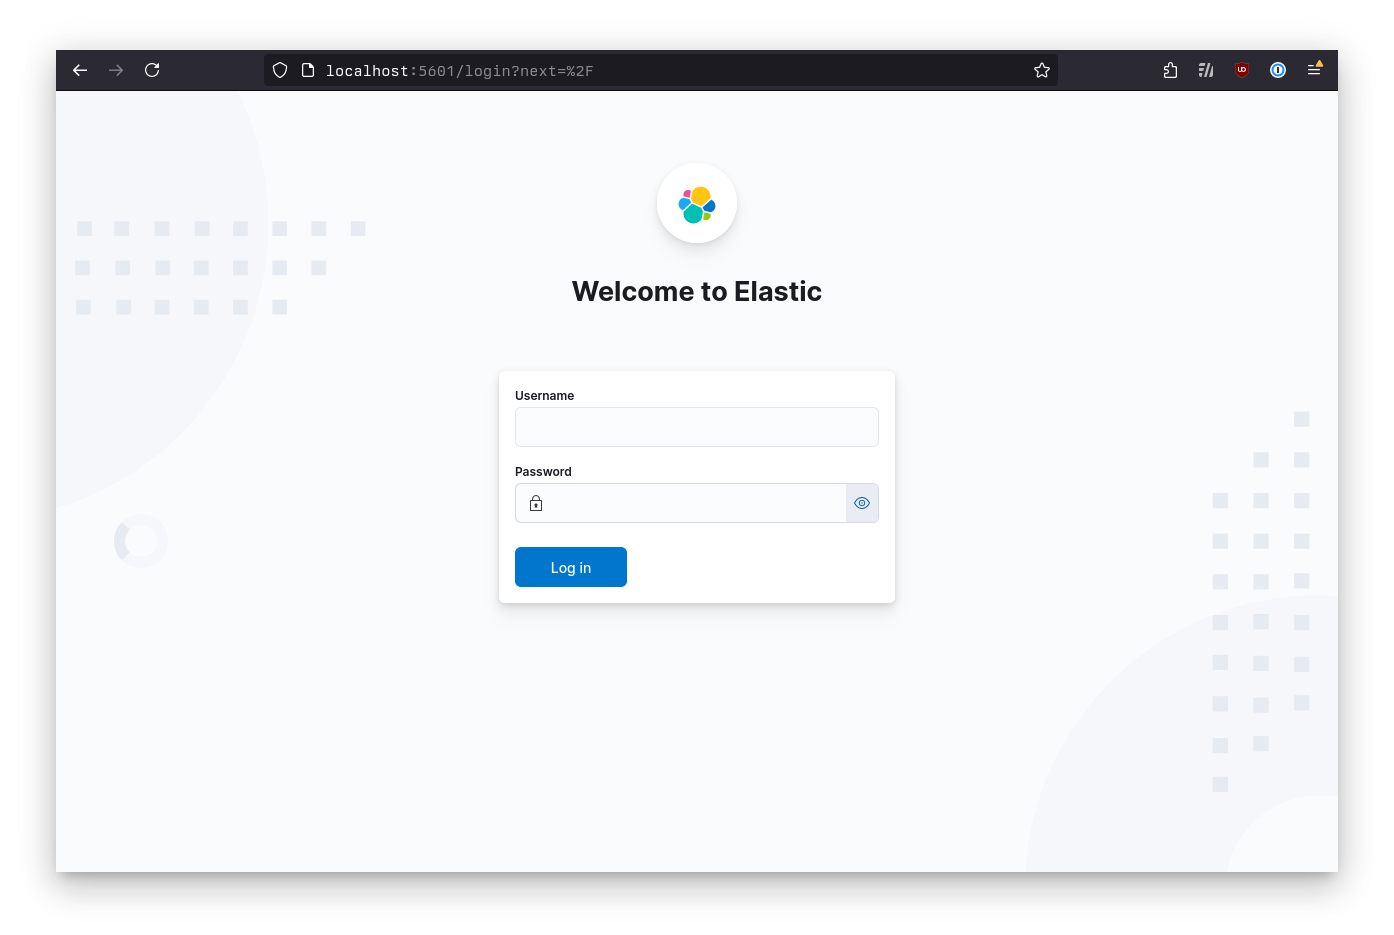
\includegraphics[width=\textwidth]{impl/local1.png}
	\caption{Inicio de sesión en Kibana}
	\label{fig:kibana_login}
\end{figure}

Una vez en la pantalla de inicio de sesión, se puede acceder con las credenciales
definidas en el archivo \texttt{.env} para el usuario \texttt{elastic}.

\begin{figure}[H]
	\centering
	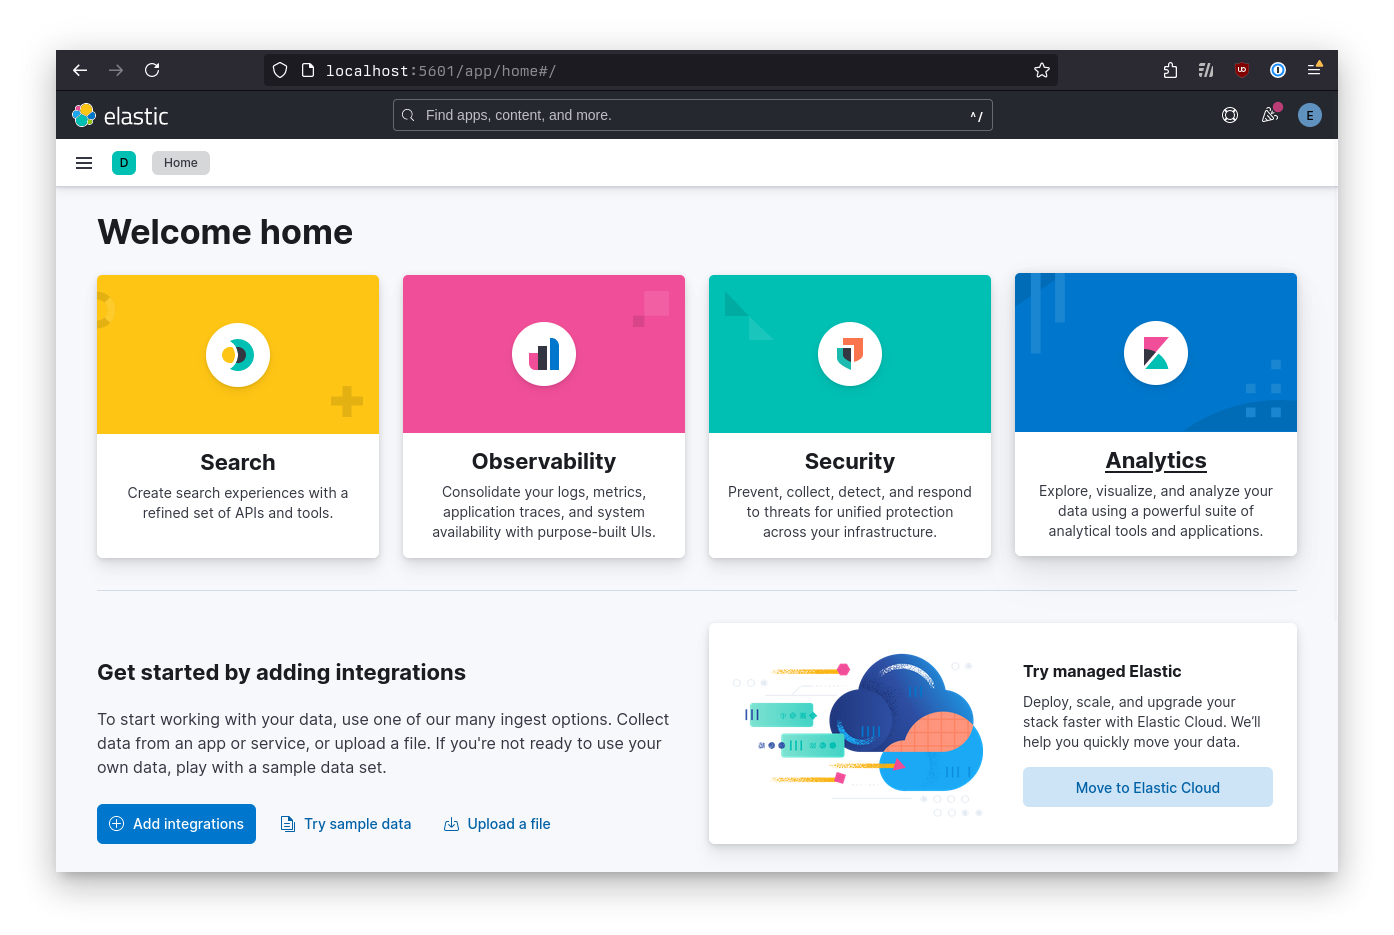
\includegraphics[width=\textwidth]{impl/local2.png}
	\caption{Página de inicio de Kibana}
	\label{fig:kibana_start}
\end{figure}

Una vez aquí, se puede hacer click en la opción \texttt{Try sample data} para
cargar un conjunto de datos de ejemplo y probar la funcionalidad de Kibana con
Elasticsearch. Por supuesto, también se pueden probar la ingesta de datos a
través de Logstash y Kafka o, si así se desea, a través de los \textit{Beats}
especializados de ingesta directa de Elastic.

Para más información, se puede consultar \fullref{sec:manual_usuario}.


\newpage{}
\subsection{Proceso de desarrollo}\label{subsec:impl_local_desarrollo}
Para el desarrollo del sistema, se ha seguido un proceso iterativo, comenzando
a partir del ejemplo oficial de Elastic para \textit{Docker Compose}\footnote{
  \url{https://www.elastic.co/blog/getting-started-with-the-elastic-stack-and-docker-compose}
}. A partir de este ejemplo, se añaden progresivamente configuraciones y
servicios, y se prueban las funcionalidades de cada uno de ellos, actualizando
con regularidad el código en el repositorio privado establecido.

\begin{figure}[H]
  \centering
  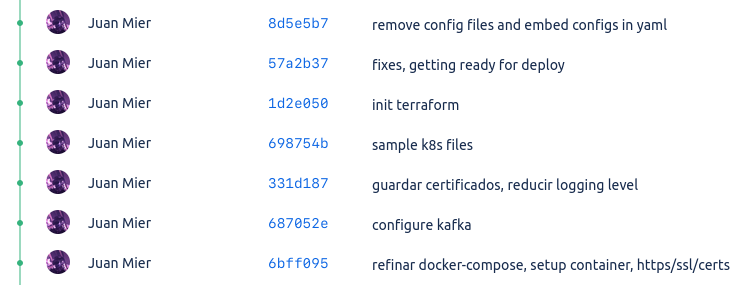
\includegraphics[width=\textwidth]{impl/commits.png}
  \caption{Ejemplo de commits en el repositorio privado}
  \label{fig:commits}
\end{figure}

Inicialmente, se prueban los servicios mínimos (Kibana y Elasticsearch) sin
HTTPS para comprobar su correcto funcionamiento. Una vez se ha comprobado que
los servicios funcionan correctamente, se añade la configuración de seguridad
y se prueban los servicios con HTTPS, ajustando más configuraciones como el
nivel de registro de logs o las comprobaciones de salud de los contenedores.

Una vez se ha comprobado que los servicios funcionan correctamente, se añaden
los servicios de Kafka, Zookeeper y Logstash, y se prueban las conexiones entre
los servicios, ajustando las configuraciones necesarias para que los servicios
se comuniquen correctamente.


\newpage{}
\section{Despliegue \textit{cloud}}\label{sec:impl_cloud}
El desarrollo principal del despliegue en la nube se concentra en la creación
de los scripts de \textit{Terraform} necesarios para la implementación de la
infraestructura planteada en el apartado \fullref{sec:arquitectura}. Para ello,
se divide el proyecto en scripts separados de manera que se puedan gestionar
los recursos y los servicios de manera independiente.

El diseño de una infraestructura base y el desarrollo de un prototipo de manera
local permiten tener una idea clara de los recursos necesarios y de las
características específicas de cada servicio, facilitándo la tarea de
desarrollo.

Para el desarollo, se hace uso de un repositorio privado en \textit{Bitbucket}
para el control de versiones y facilitar a la empresa la revisión y uso del
código. El código completo se encuentra en \fullref{anexo:cloud}.

Esta sección de la memoria documenta el desarrollo de las siguientes historias
de usuario, siguiendo la planificación establecida en la sección \fullref{sec:planif_inicial}:

\begin{table}[H]
	\centering
	\begin{tabular}{|p{0.7\linewidth}|c|c|}
		\hline
		\textbf{Nombre} & \textbf{Prioridad} & \textbf{Tamaño} \\
		\hline
		\hline
		Como desarrollador de Okticket, quiero que la arquitectura se despliegue y orqueste de manera automática & P0\cellcolor{red!50} & XL\cellcolor{red!50} \\
		\hline
  \end{tabular}
  \caption{Lista de HUs cumplimentadas con el despliegue en la nube}
  \label{tab:impl_cloud}
\end{table}


\newpage{}
\subsection{Proceso de desarrollo}\label{subsec:impl_cloud_desarrollo}
El proceso de desarrollo de los scripts de \textit{Terraform} parte de la
implementación original de la infraestructura en local, y se va adaptando a
las necesidades de la infraestructura en la nube, puesto que ambos comparten
similaridades (como la mayoría de la configuración de los servicios, la
estructura general de los mismos, las imágenes y versiones utilizadas, etc.).

Al igual que con el desarrollo local, se sigue un proceso iterativo, comenzando
por la creación de un solo servicio, en este caso Kafka, y continuando con el
resto de la arquitectura. Los primeros despliegues son tan solo pruebas de
concepto, con el objetivo de adaptarse a la infraestructura de la nube, el
funcionamiento de Terraform y la configuración de AWS.

Pese a que Terraform suele encargarse de la creación, modificación y destrucción
de los recursos de manera automática, existen casos en los que es necesaria la
intervención manual, como en la destrucción de los contenedores de
\textit{Secret Manager} o en la actualización de algunas configuraciones de los
recursos. Estos casos ocurrirán solo durante la fase de desarrollo, puesto que
se espera que, en la fase de producción, no sea necesario la reconfiguración de
los recursos y servicios.

La definición de las tareas de ECS durante el desarrollo queda registrado en la
sección correspondiente de AWS, cuyo código y configuraciones se puede consultar
si así se desea.

\begin{figure}[H]
	\centering
	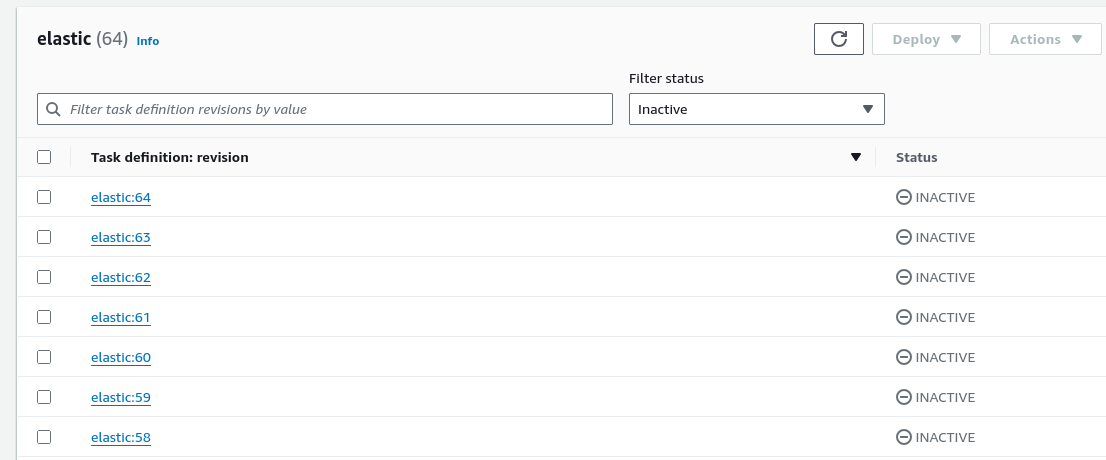
\includegraphics[width=\textwidth]{impl/definitions.png}
	\caption{Ejemplo de definciones de tareas de ECS en AWS}
	\label{fig:definitions}
\end{figure}

\begin{figure}[H]
	\centering
	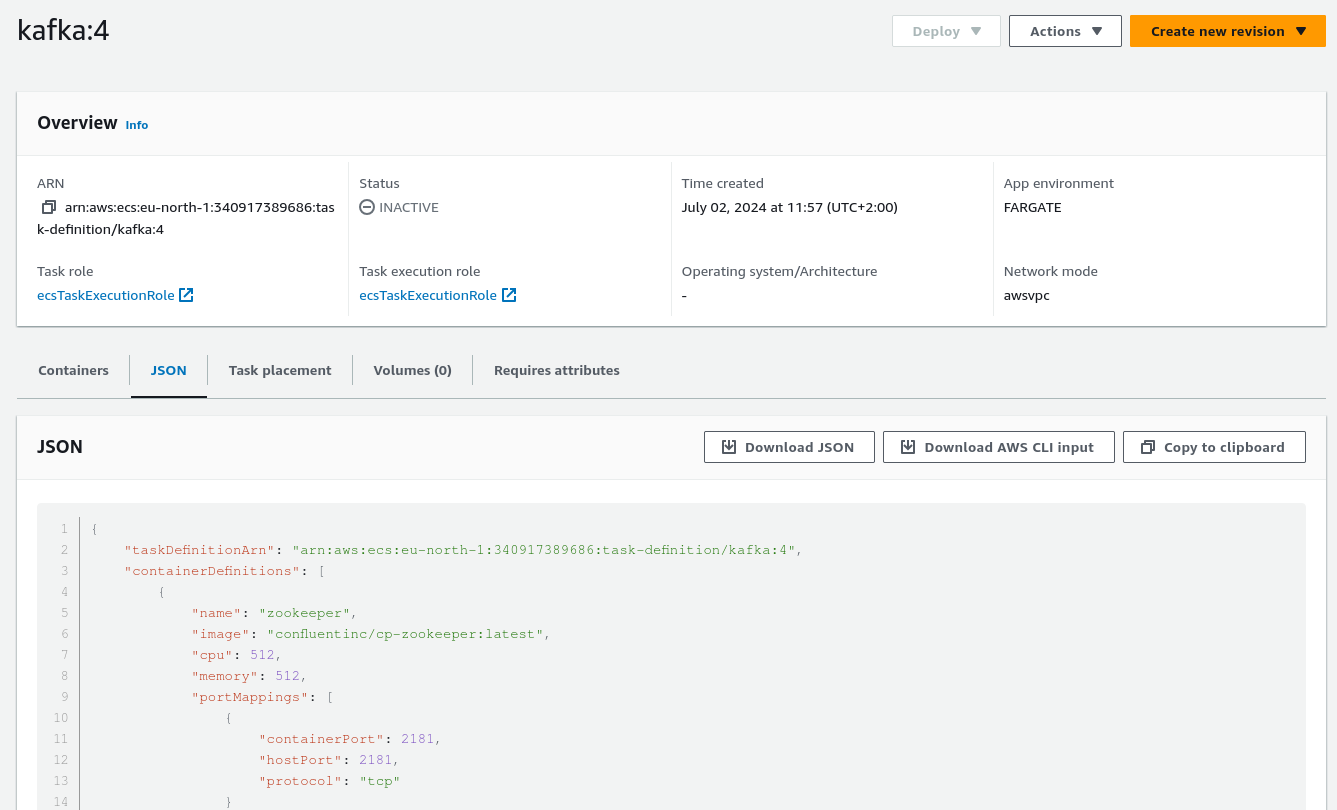
\includegraphics[width=\textwidth]{impl/ejemplo_definition.png}
	\caption{Ejemplo de definción de tarea (Kafka)}
	\label{fig:definition}
\end{figure}

Durante el desarrollo del despliegue, se utilizan las herramientas de
monitorización de AWS para comprobar el estado de los recursos y servicios
creados, y se realizan pruebas básicas de funcionamiento para asegurar que los
servicios se han desplegado correctamente. En la figura \ref{fig:task_logs}, se muestran
los logs de una tarea de ECS.

\begin{figure}[H]
	\centering
	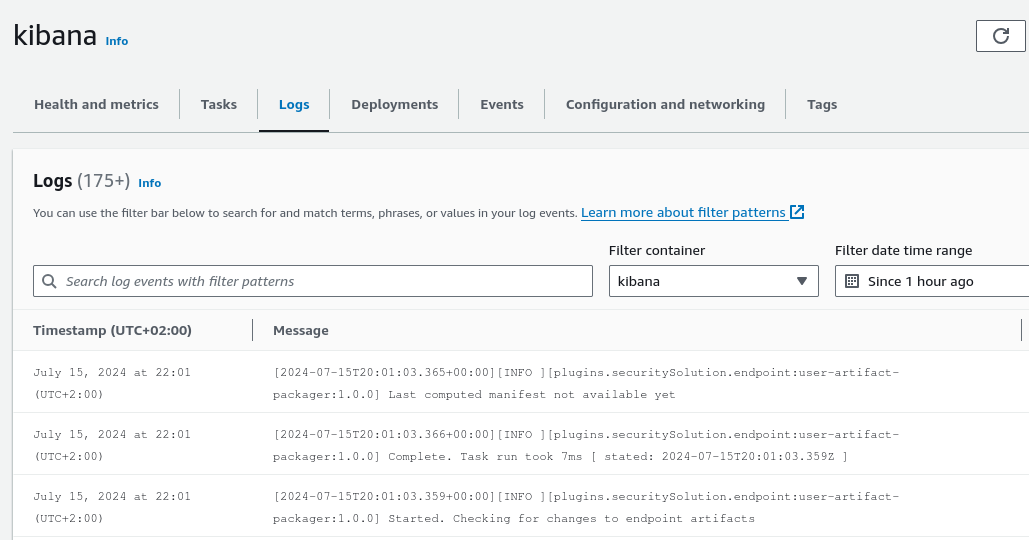
\includegraphics[width=\textwidth]{impl/task_logs.png}
	\caption{Ejemplo de logs de una tarea de ECS}
	\label{fig:task_logs}
\end{figure}

En la figura \ref{fig:estado_elb}, se muestra el estado actual de todos los balanceadores
de carga, junto a más detalles como sus zonas de disponibilidad o el estado de
los nodos.

\begin{figure}[H]
	\centering
	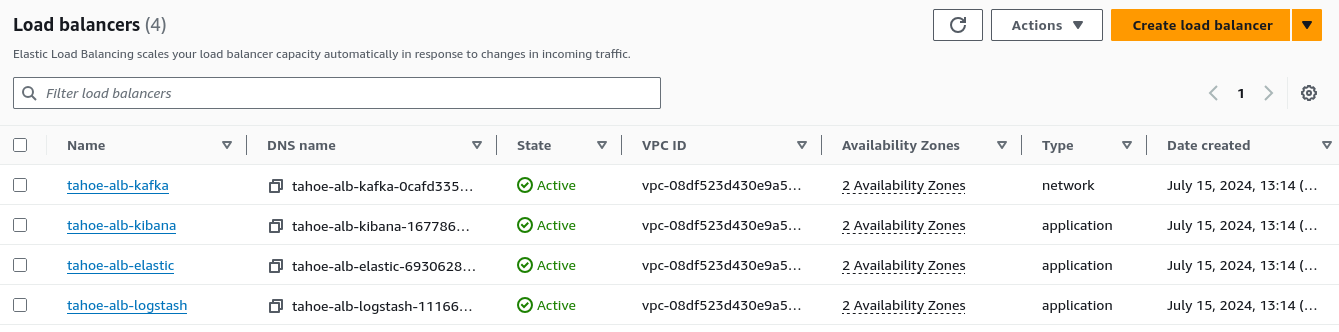
\includegraphics[width=\textwidth]{impl/estado_elb.png}
	\caption{Estado de los balanceadores de carga}
	\label{fig:estado_elb}
\end{figure}

Por último, en la figura \ref{fig:deploy_state} se muestra el estado de un
despliegue de un servicio, con información sobre el estado de los contenedores,
la versión de la imagen, la cantidad de tareas en ejecución y la cantidad de
tareas deseadas.

\begin{figure}[H]
	\centering
	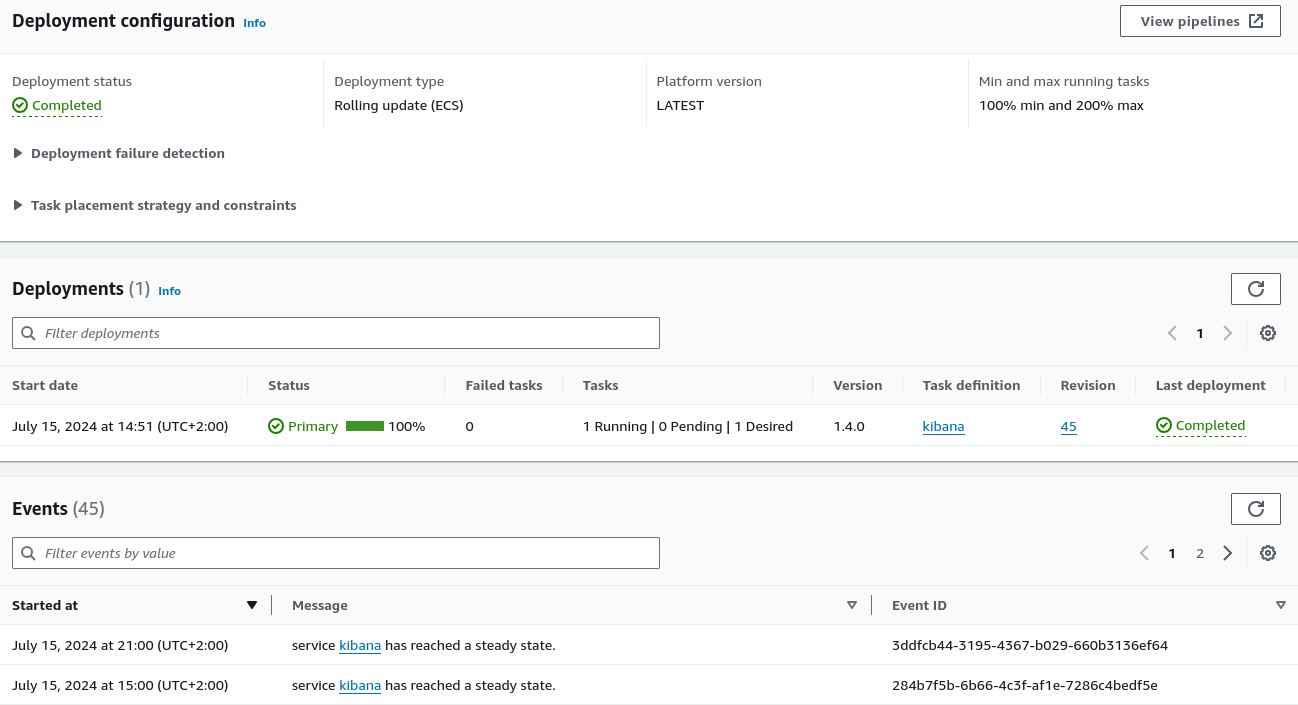
\includegraphics[width=\textwidth]{impl/deploy_state.png}
	\caption{Métricas de estado del despliegue de un servicio}
	\label{fig:deploy_state}
\end{figure}

Por supuesto, los propios servicios cuentan con sus herramientas de
monitorización básicas a las que se puede acceder a través del navegador (en
caso de que funcionen correctamente).

\begin{figure}[H]
	\centering
	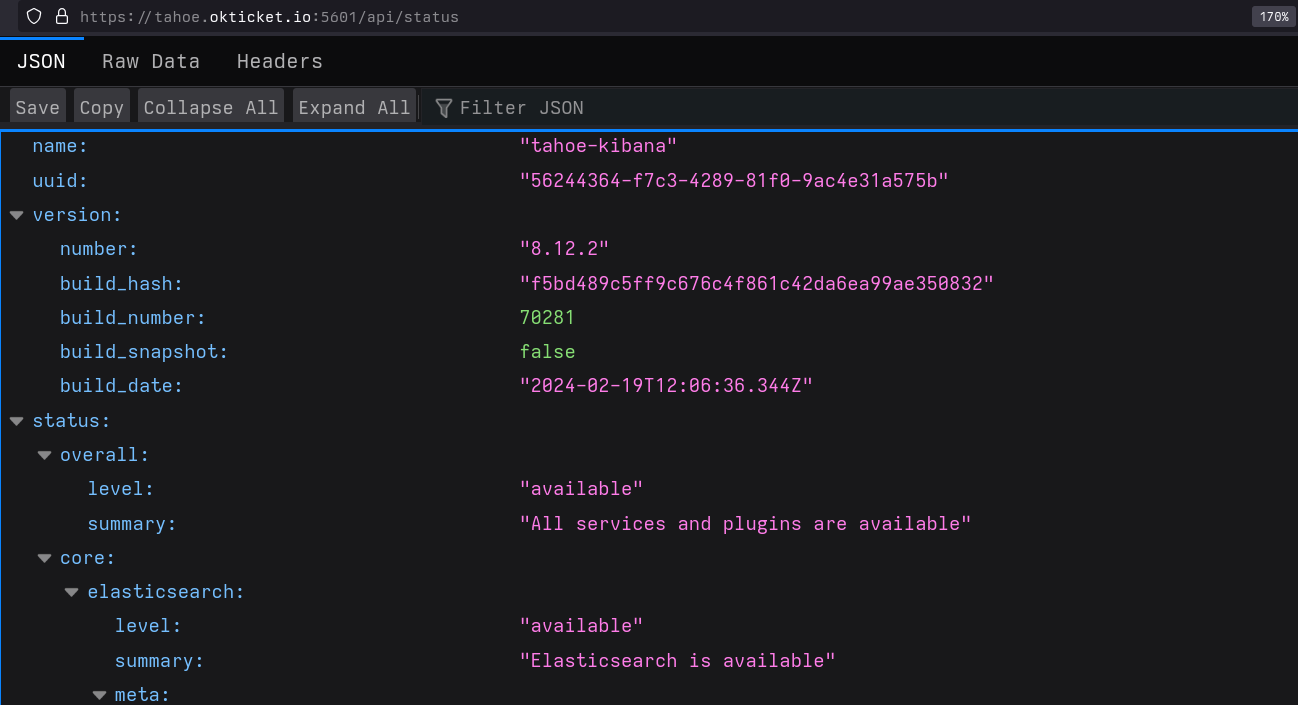
\includegraphics[width=\textwidth]{impl/kibana_status.png}
	\caption{Estado de Kibana}
	\label{fig:kibana_status}
\end{figure}

Estas herramientas se utilizan para el desarrollo incremental y la comprobación
de que los servicios se despliegan correctamente, y se espera que, en la fase de
producción, no sea necesario su uso, puesto que se cuenta con herramientas de
monitorización más avanzadas y específicas para cada servicio.

\newpage{}
\subsection{Despliegue de la infraestructura}\label{subsec:impl_cloud_despliegue}
% TODO: desarrollar
% Aquí podría estar bien poner un diagrama de despliegue. Pero que se vea en el
% modelo que ese diagrama de despliegue no es el despliegue de tu proyecto.
% Es decir, el proyecto es crear un proceso de despliegue que hace un despliegue.
% Entonces que se vea que hay ese proceso y luego el diagrama de despliegue de lo
% que el proyecto permite desplegar
Para desplegar la infraestructura diseñada en AWS utilizando Terraform, se
siguen los siguientes pasos:

\begin{enumerate}
    \item \textbf{Preparación del entorno:} Asegurarse de tener instalado
    Terraform y configuradas las credenciales de AWS correctamente.

    \item \textbf{Inicialización:} Ejecutar el comando \texttt{terraform init}
    en el directorio que contiene los archivos de configuración de Terraform.
    Esto descarga los proveedores necesarios y inicializa el estado de
    Terraform.

    \item \textbf{Planificación:} Utilizar el comando \texttt{terraform plan}
    para revisar los cambios que Terraform realizará en la infraestructura.
    Este paso ayuda a identificar posibles problemas antes de aplicar los
    cambios.

    \item \textbf{Aplicación:} Ejecutar \texttt{terraform apply} para crear o
    modificar la infraestructura en AWS según la configuración definida.
    Terraform solicitará confirmación antes de realizar cambios.

    \item \textbf{Verificación:} Una vez completado el despliegue, verificar
    en la consola de AWS que todos los recursos se han creado correctamente.
    Comprobar que los servicios (Elasticsearch, Kibana, Logstash, Kafka) están
    en funcionamiento y accesibles.

    \item \textbf{Pruebas:} Realizar pruebas básicas de conectividad y
    funcionalidad para asegurar que la infraestructura está operativa y
    cumple con los requisitos establecidos.
\end{enumerate}

Como se ha mencionado anteriormente, durante cualquier fase del despliegue
pueden ocurrir erorres o problemas que requieran intervención manual. En caso
de que ocurran, se debe revisar el estado de los recursos y servicios en la
consola de AWS, y se debe corregir el problema manualmente si es necesario.

Se mantiene un control de versiones de los archivos de
configuración de Terraform para facilitar el seguimiento de cambios y la
posible futura colaboración en el desarrollo de la infraestructura.

Para visualizar el proceso de despliegue de la infraestructura, se ha creado
un diagrama que ilustra los principales componentes y pasos. Este diagrama se
muestra en la Figura \ref{fig:deployment-diagram}.

\begin{figure}[H]
    \centering
    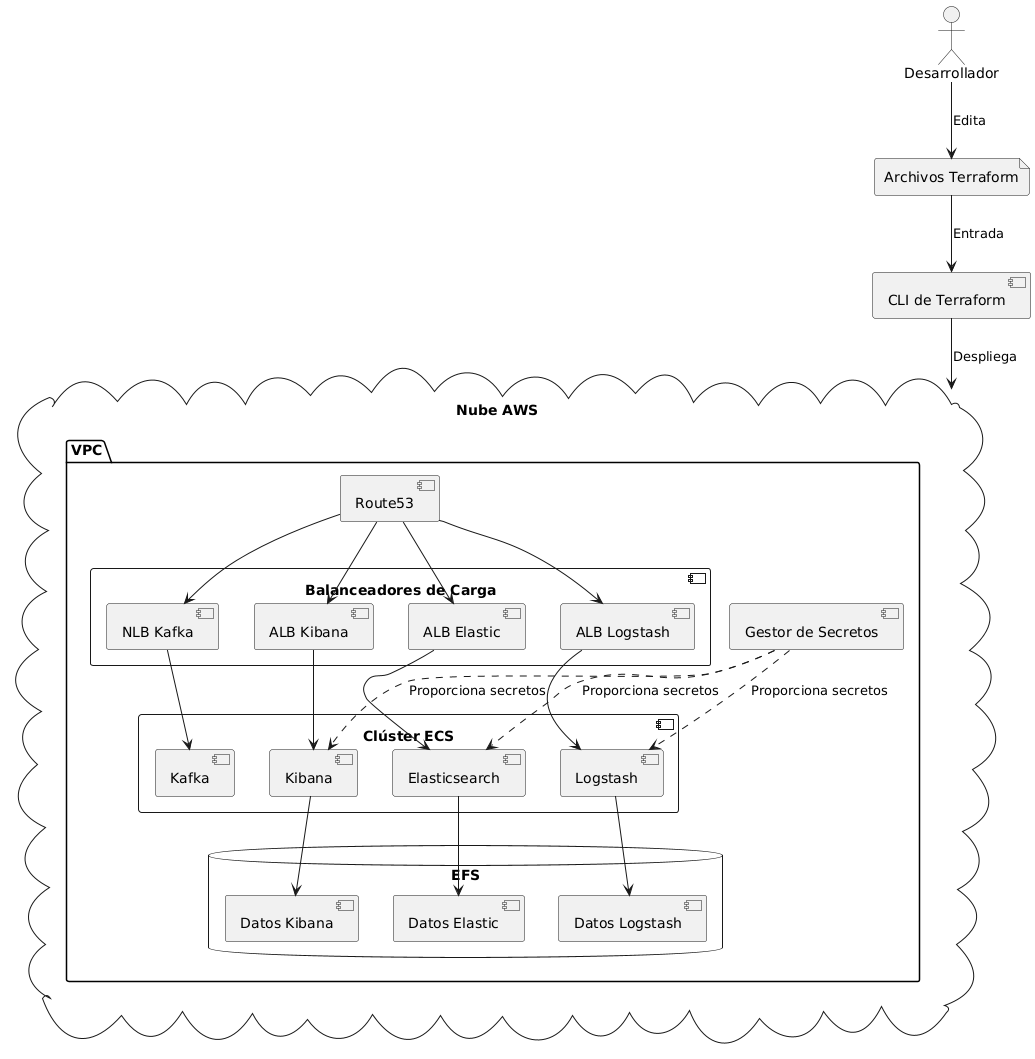
\includegraphics[width=\textwidth]{uml/deploy.png}
    \caption{Diagrama de despliegue de la infraestructura}
    \label{fig:deployment-diagram}
\end{figure}

El diagrama muestra el flujo desde los archivos de configuración de Terraform
hasta los recursos desplegados en AWS, pasando por las diferentes etapas del
proceso de despliegue.


\newpage{}
\subsection{Explicación del código}\label{sec:impl_configuracion}
\emph{El código completo se encuentra en el anexo \fullref{anexo:cloud}.}

Los scripts de Terraform se dividen en varios archivos, cada uno de ellos con
una función específica, con el objetivo de facilitar la gestión y configuración
de los recursos y servicios. A continuación, se detallan dichos archivos y su
función en el proyecto.


\subsubsection{Recursos generales}
Como previamente descrito, la definción de los recursos generales se divide en
ficheros, cada uno de ellos con una función específica. A continuación, se
detallan dichos ficheros y su función en el proyecto.


\paragraph{Fichero principal}
El fichero principal de Terraform, \halfref{lst:main}{main.tf}, se encarga de
las configuraciones más esenciales o que no tienen cabida en otros ficheros,
como la definción de la región, el cluster, el grupo de logs o el bucket S3 de
logs.


\paragraph{Variables}
El fichero de variables \halfref{lst:variables}{variables.tf}
se encarga de la definición de todas las variables necesarias para el despliegue
de la infraestructura, como nombres, regiones, versiones, puertos, etc., de
manera que se puedan modificar y
reutilizar de manera sencilla a lo largo del resto de ficheros de definción.

También se definen contraseñas de manera aleatoria, para mejorar la seguridad
de los servicios.


\paragraph{Salidas}
El fichero de salidas \halfref{lst:outputs}{outputs.tf} se encarga de la
definición de las salidas de Terraform, es decir, de las variables que se pueden
consultar una vez que se ha desplegado la infraestructura, como las direcciones
URL de los servicios o las contraseñas generadas alteatoriamente.

Un ejemplo de estas salidas se encuentra en la figura
\fullref{fig:terraform_output}.


\newpage{}
\paragraph{Volúmenes lógicos (EFS)}
El fichero de volúmenes lógicos \halfref{lst:efs}{efs.tf} se encarga de la
definción de los volúmenes lógicos necesarios para la persistencia de los datos
de los servicios, como los datos de Elasticsearch o los logs de los servicios.


\paragraph{Roles, políticas y permisos (IAM)}
El fichero de roles, políticas y permisos \halfref{lst:iam}{iam.tf} se encarga
de la definción de los roles y políticas necesarios para el correcto
funcionamiento de los servicios, como los roles de ejecución de tareas de ECS,
los permisos de acceso a los servicios de AWS o las políticas de acceso a los
recursos.


\paragraph{Secretos}
El fichero de secretos \halfref{lst:secrets}{secrets.tf} se encarga de la
definción de las claves necesarias para el correcto funcionamiento de los
servicios, como los certificados de Elasticsearch o las claves de acceso a los
servicios.

Estos secretos se almacenan en \textit{AWS Secrets Manager}, un servicio de AWS
que permite el almacenamiento seguro de información sensible, como contraseñas,
claves de acceso o certificados. Los certificados se almacenan en formato
\texttt{base64} para facilitar su almacenamiento y evitar problemas de
codificación en el paso de los mismos. Se utilizan cadenas generadas
aleatoriamente para evitar la exposición de contraseñas y claves de acceso en el
código.


\paragraph{Redes}
El fichero de redes \halfref{lst:network}{network.tf} se encarga de la definción
de los elementos de red necesarios para la correcta comunicación entre los
servicios y su seguridad.

La lógica y arquitectura de red se explica en el apartado
\fullref{subsec:redes}, lo que facilita la definición de las redes en Terraform.


\paragraph{Grupos de seguridad}
El fichero de grupos de seguridad \halfref{lst:security}{security.tf} se encarga
de la definción de los grupos de seguridad necesarios para la correcta
comunicación entre los servicios y su seguridad.

La lógica y arquitectura de seguridad se explica en el apartado
\fullref{subsec:seguridad}.


\newpage{}
\subsubsection{Servicios de ELK}
Puesto que la estructura de definción de servicios en Terraform es similar para
todos los servicios, se analiza el más completo, Elasticsearch, para explicar el
funcionamiento y la lógica de los mismos.

Cada fichero de definción de servicios está separado en tres partes:
\begin{enumerate}
	\item \textbf{Definción de la tarea}, que contiene la configuración del
		contenedor al estilo de \textit{Docker Compose} (imagen, variables de
    entorno, volúmenes, etc.)
	\item \textbf{Definción del servicio}, que asigna la tarea al resto de la
		configuración del servicio.
	\item \textbf{Definción de recursos}, los necesarios para cada servicio:
		balanceadores de carga, \textit{listeners}, configuraciones DNS, etc.
\end{enumerate}

El código completo de los servicios se encuentra en el anexo \fullref{anexo:cloud}.

\paragraph{Definción de la tarea}
A continuación, se muestra un ejemplo de la definción de la tarea de Elastic:

\begin{lstlisting}[caption={Definción de la tarea de Elastic}, label={lst:elastic_task}]
	resource "aws_ecs_task_definition" "elastic" {
  family                   = "elastic"
  network_mode             = "awsvpc"
  requires_compatibilities = [var.launch_type]
  cpu                      = "2048"
  memory                   = "4096"
  execution_role_arn       = aws_iam_role.ecs_task_execution.arn
  task_role_arn            = aws_iam_role.ecs_task_execution.arn

  container_definitions = jsonencode([
    {
      name      = "es01"
      image     = "docker.elastic.co/elasticsearch/elasticsearch:${var.stack_version}"
      cpu       = 2048
      memory    = 4096
      essential = true
      environment = [
        { name = "cluster.name", value = var.cluster_name },
        { name = "xpack.security.enabled", value = "true" },
        { name = "xpack.security.http.ssl.enabled", value = "true" },
		<...>
      ]
      secrets = [
        {
          name      = "CA_CRT"
          valueFrom = "${aws_secretsmanager_secret.es_certs.arn}:ca.crt::"
        },
        {
          name      = "ES01_KEY"
          valueFrom = "${aws_secretsmanager_secret.es_certs.arn}:es01.key::"
        },
        <...>
      ]
      entrypoint = [
        "/bin/sh",
        "-c",
        <<-EOT
        #!/bin/bash
        set -e

        echo "Configurando credenciales..."
        mkdir -p /usr/share/elasticsearch/config/certs
        echo $CA_CRT | base64 -d > /usr/share/elasticsearch/config/certs/ca.crt
        <...>
        EOT
      ]
      # mountPoints = [
      #   {
      #     sourceVolume  = "elastic-data"
      #     containerPath = "/usr/share/elasticsearch/data"
      #     readOnly      = false
      #   }
      # ]
      portMappings = [
        {
          containerPort = var.elastic_port,
          hostPort      = var.elastic_port
        }
      ]
      logConfiguration = {
        logDriver = var.log_driver
        options = {
          "awslogs-group"         = var.log_group
          "awslogs-region"        = var.region
          "awslogs-stream-prefix" = "elastic"
        }
      }
      ulimits = [
        {
          name      = "memlock"
          softLimit = -1
          hardLimit = -1
        },
        {
          name      = "nofile"
          softLimit = 65536
          hardLimit = 65536
        }
      ]
    }
  ])

  volume {
    name = "elastic-data"
    efs_volume_configuration {
      file_system_id = aws_efs_file_system.elastic_data.id
      root_directory = "/"
    }
  }
}
\end{lstlisting}

Como se puede comprobar, pese a que la sintaxis de configuración es distinta,
la estructura de la misma es muy similar a aquella ya definida durante el
\fullref{sec:impl_local}, con similares configuraciones de entorno, mapeos de
puertos y volúmenes, y configuraciones de red. Ese es el objetivo del
planteamiento iterativo y de desarrollo incremental, que permite reutilizar
código y configuraciones ya definidas.

Al igual que en el desarrollo local, se obvia la configuración de los recursos
necesaria para la escalabilidad y replicación de los servicios, puesto que de
momento no se necesitan más que una instancia de cada servicio. Sin embargo,
esto no significa que no se pueda añadir de manera sencilla en un futuro, como
así lo demuestran, por ejemplo, la asignación de los servicios a volúmenes EFS.

A diferencia del desarrollo local, la preparación del servicio se realiza desde
la clave de configuración \texttt{entrypoint}, en lugar de requerir un segundo
contenedor de configuración.


\newpage{}
\paragraph{Definción del servicio}
A continuación, se detalla la definición del servicio de Elasticsearch:

\begin{lstlisting}[caption={Definción del servicio de Elastic}, label={lst:elastic_service}]
	resource "aws_ecs_service" "elastic" {
  name                   = "elastic"
  cluster                = aws_ecs_cluster.cluster.id
  task_definition        = aws_ecs_task_definition.elastic.arn
  desired_count          = 1
  launch_type            = var.launch_type
  enable_execute_command = true

  network_configuration {
    subnets          = [aws_subnet.private.id]
    security_groups  = [aws_security_group.elastic.id]
    assign_public_ip = true
  }

  load_balancer {
    target_group_arn = aws_lb_target_group.elastic.arn
    container_name   = "es01"
    container_port   = var.elastic_port
  }

  depends_on = [
    aws_lb_listener.elastic,
    aws_ecs_task_definition.elastic
  ]
}
\end{lstlisting}

La definción del servicio es mucho más breve que el resto de definiciones,
puesto que la mayoría de la configuración se realiza en la tarea. En este caso,
se asigna la tarea a un grupo de seguridad y a una subred privada, y se asigna
el servicio a un balanceador de carga, que se encargará de distribuir el tráfico
entre los contenedores.


\newpage{}
\paragraph{Definción de recursos}
Todos los recursos necesarios para el servicio, como el balanceador de carga, el
grupo de seguridad, el \textit{listener} o la configuración DNS, se definen a
continuación.

\begin{lstlisting}[caption={Definción de recursos de Elastic}, label={lst:elastic_resources}]
resource "aws_lb" "elastic" {
  name               = "tahoe-alb-elastic"
  internal           = false
  load_balancer_type = "application"
  security_groups    = [aws_security_group.elastic.id]
  subnets            = [aws_subnet.public_a.id, aws_subnet.public_b.id]

  access_logs {
    bucket  = aws_s3_bucket.access_logs.bucket
    prefix  = "elastic"
    enabled = true
  }
}

resource "aws_lb_target_group" "elastic" {
  name        = "tahoe-tg-elastic"
  port        = var.elastic_port
  protocol    = "HTTPS"
  vpc_id      = aws_vpc.main.id
  target_type = "ip"

  health_check {
    enabled             = true
    path                = "/"
    protocol            = "HTTPS"
    matcher             = "200"
    interval            = 300
    timeout             = 60
    healthy_threshold   = 2
    unhealthy_threshold = 5
    port                = tostring(var.elastic_port)
  }
}

resource "aws_lb_listener" "elastic" {
  load_balancer_arn = aws_lb.elastic.arn
  port              = var.elastic_port
  protocol          = "HTTPS"
  ssl_policy        = "ELBSecurityPolicy-2016-08"
  certificate_arn   = aws_acm_certificate.elastic.arn

  default_action {
    type             = "forward"
    target_group_arn = aws_lb_target_group.elastic.arn
  }
}

resource "aws_lb_listener" "elastic_https" {
  load_balancer_arn = aws_lb.elastic.arn
  port              = 443
  protocol          = "HTTPS"
  ssl_policy        = "ELBSecurityPolicy-2016-08"
  certificate_arn   = aws_acm_certificate.elastic.arn

  default_action {
    type = "redirect"
    redirect {
      port        = tostring(var.elastic_port)
      protocol    = "HTTPS"
      status_code = "HTTP_301"
    }
  }
}

resource "aws_acm_certificate" "elastic" {
  domain_name       = local.elastic_url
  validation_method = "DNS"

  lifecycle {
    create_before_destroy = true
  }
}

resource "aws_route53_record" "elastic" {
  zone_id = var.route53_zone_id
  name    = local.elastic_url
  type    = "A"

  alias {
    name                   = aws_lb.elastic.dns_name
    zone_id                = aws_lb.elastic.zone_id
    evaluate_target_health = false
  }
}

resource "aws_route53_record" "elastic_validation" {
  for_each = {
    for dvo in aws_acm_certificate.elastic.domain_validation_options : dvo.domain_name => {
      name   = dvo.resource_record_name
      record = dvo.resource_record_value
      type   = dvo.resource_record_type
    }
  }

  allow_overwrite = true
  name            = each.value.name
  records         = [each.value.record]
  ttl             = 60
  type            = each.value.type
  zone_id         = var.route53_zone_id
}

resource "aws_acm_certificate_validation" "elastic" {
  certificate_arn         = aws_acm_certificate.elastic.arn
  validation_record_fqdns = [for record in aws_route53_record.elastic_validation : record.fqdn]
}
\end{lstlisting}

Como para todos los servicios, se necesitan definir los recursos de red que
permitan acceder a los mismos, es decir:

\begin{itemize}
	\item Un balanceador de carga que distribuya el tráfico entre los
		contenedores de Elasticsearch.
	\item Un \textit{target group} que asigne los contenedores al balanceador de
		carga y permita la comprobación de la salud de los contenedores.
	\item \textit{Listeners} que permitan el acceso a los servicios desde el
		exterior o redirijan el tráfico a los contenedores dependiendo del
		puerto de conexión.
\end{itemize}

En el caso de Elastic (y el de otros servicios como Kibana), también se requiere
la configuración de un subdominio DNS y sus certificados pertinentes, para
facilitar el acceso a los servicios desde el exterior. Sin dichos subdominios,
la dirección URL de los servicios cambiaría cada vez que se desplegaran, lo que
dificultaría el acceso a los mismos. El tiempo de vida (\textit{TTL}) de estas
definiciones es de un minuto por defecto, lo que permite la actualización de
los certificados y la dirección URL de manera rápida y sencilla.


\newpage{}
\section{Ingesta de datos}\label{sec:impl_ingesta}
Tras la creación y el despliegue de la infraestructura base, se procede a la
creación de los scripts de ingesta de datos, de manera escalonada y siguiendo
la prioridad de las fuentes de datos.

Esta sección de la memoria documenta el desarrollo de las siguientes historias
de usuario, siguiendo la planificación establecida en la sección \fullref{sec:planif_inicial}:

\begin{table}[H]
	\centering
	\begin{tabular}{|p{0.7\linewidth}|c|c|}
		\hline
		\textbf{Nombre} & \textbf{Prioridad} & \textbf{Tamaño} \\
		\hline
		\hline
		Como desarrollador de Okticket, quiero que se ingesten de manera automática datos de la base de datos interna de MongoDB & P0\cellcolor{red!50} & M\cellcolor{yellow!50} \\
		\hline
		Como desarrollador de Okticket, quiero que se ingesten de manera automática datos de la base de datos interna de MySQL & P0\cellcolor{red!50} & M\cellcolor{yellow!50} \\
		\hline
		Como desarrollador de Okticket, quiero que los datos se limpien de manera automática & P0\cellcolor{red!50} & S\cellcolor{green!25} \\
		\hline
		Como desarrollador de Okticket, quiero que se ingesten de manera automática logs de balanceador de AWS & P1\cellcolor{orange!50} & M\cellcolor{yellow!50} \\
		\hline
  \end{tabular}
  \caption{Lista de HUs cumplimentadas con la ingesta de datos}
  \label{tab:impl_ingesta}
\end{table}


\newpage{}
\subsection{Ingesta de métricas con Kafka}\label{subsec:impl_ingesta_kafka}
Puesto que se ha decidido utilizar Kafka como sistema de mensajería, se
desarrollan los scripts de ingesta de datos para que los datos se envíen a
Kafka y se procesen mediante Logstash y Elasticsearch.

Para la ingesta de datos, se han desarrollado scripts de Python que se encargan
de la lectura de los datos de las fuentes, su transformación y su envío a Kafka.
Estos scripts se ejecutan en bucle con una parada de segundos entre ejecuciones,
aunque se pueden adaptar para cualquier otra ejecución periódica como triggers,
\textit{cron jobs} o \textit{webhooks}.

Algunos de los servidores que contienen la información a ingestar se encuentran
detrás de subredes privadas, por lo que los scripts de ingesta se deben ejecutar
a través de \texttt{SSH} en los servidores bastiones de dichas subredes. Estos
servidores se encargarán de conectar con la infraestructura desplegada y enviar
la información.

\textit{Ver código: \fullref{anexo:kafka}}


\subsubsection{Componentes de Kafka}
\textit{Kafka} se compone de varios componentes clave:

\begin{itemize}
    \item \textbf{Tópico}: Un tópico es una categoría a la que se envían los
		mensajes y a la que los consumidores están \textit{suscritos}. Los
		consumidores pueden estar suscritos a uno o varios tópicos, y los
		productores pueden enviar mensajes a uno o varios tópicos. Los tópicos
		son la unidad básica de organización de los mensajes en cualquier
		sistema de mensajería de publicación/suscripción.
    \item \textbf{Productor}: El productor es el componente responsable de crear
		y enviar mensajes al cluster de Kafka. Está separado del resto de los
		componentes y produce mensajes de manera asíncrona y rápida.
    \item \textbf{Consumidor}: El consumidor es el componente responsable de
		leer los mensajes producidos por el productor. Está suscrito a un tópico
		a través del broker y consume los mensajes.
    \item \textbf{Broker}: El broker es el componente responsable de recibir los
		mensajes producidos por el productor y enviarlos a los consumidores. Es
		el intermediario entre los productores y los consumidores.
\end{itemize}


\newpage{}
\subsubsection{Explicación del código}
Todos los \textit{productores} de datos siguen un patrón similar, ya que su
función es la misma: leer datos de una fuente, transformarlos y enviarlos a
Kafka.

Su código se divide en tres partes principales, siguiendo con el patrón de
diseño de \textit{Extract, Transform, Load} (ETL) definido anteriormente
(ver~\ref{sec:etl}):

\begin{itemize}
	\item \textbf{Lectura de datos:} se encarga de la lectura de los datos de
		la fuente de datos. En el caso de las bases de datos, se conecta a la
		base de datos y ejecuta una consulta para obtener los datos. En el caso
		de los logs, se lee el fichero de logs y se extraen las líneas que
		contienen la información necesaria.
	\item \textbf{Transformación de datos:} se encarga de la transformación de
		los datos leídos a un formato adecuado para su envío a Kafka. En el caso
		de las bases de datos, se transforman los datos a un formato JSON. En el
		caso de los logs, se transforman las líneas de logs a un formato JSON.
	\item \textbf{Envío de datos:} se encarga del envío de los datos a Kafka.
		Para ello, se conecta a Kafka y envía los datos a un tópico concreto.
\end{itemize}


\subsubsection{Dependencias}
Para la ejecución de los scripts de Python, se necesitan las siguientes
librerías, dependiendo del script a ejecutar:

\begin{itemize}
	\item \textbf{kafka-python:} librería de Python que permite la conexión y
		el envío de datos a Kafka.
	\item \textbf{pymsql:} librería de Python que permite la conexión y la
		ejecución de consultas en bases de datos MySQL.
	\item \textbf{pymongo:} librería de Python que permite la conexión y la
		ejecución de consultas en bases de datos MongoDB.
	\item \textbf{python-dotenv:} librería de Python que permite la carga de
		variables de entorno desde un fichero \texttt{.env}.
\end{itemize}


\newpage{}
\subsection{Ingesta de logs de AWS}\label{subsec:impl_ingesta_aws}
Para la ingesta de logs de balanceadores de carga de AWS, se desarrolla una
lambda en Python que se encarga de la lectura de los logs de CloudWatch y su
envío a Logstash. Se siguen cuatro pasos principales:

\begin{enumerate}
	\item \textbf{Creación de la lambda:} se crea una lambda en Python que se
		ejecuta cada vez que se genera un log en CloudWatch (5 minutos)
	\item \textbf{Filtro de subscripción:} se crea una suscripción en CloudWatch
		para que los logs generados se envíen a la lambda.
	\item \textbf{Configuración de Logstash:} se configura Logstash para que
		reciba los logs de la lambda y los envíe a Elasticsearch.
	\item \textbf{Creación del índice:} se crea un índice en Elasticsearch para
		almacenar los logs.
\end{enumerate}

\begin{figure}[h]
	\centering
	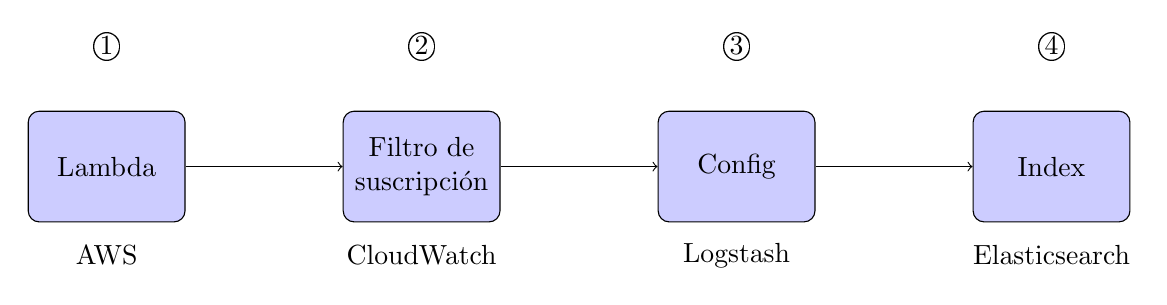
\begin{tikzpicture}[node distance=2cm, auto]
		% Definición de estilos
		\tikzstyle{block} = [rectangle, draw, fill=blue!20,
			text width=5em, text centered, rounded corners, minimum height=4em]
		\tikzstyle{line} = [draw, ->]

		% Nodos
		\node [block] (lambda) {Lambda};
		\node [block, right of=lambda, node distance=4cm] (filtro) {Filtro de suscripción};
		\node [block, right of=filtro, node distance=4cm] (logstash) {Config};
		\node [block, right of=logstash, node distance=4cm] (indice) {Index};

		% Conexiones
		\path [line] (lambda) -- (filtro);
		\path [line] (filtro) -- (logstash);
		\path [line] (logstash) -- (indice);

		% Etiquetas
		\node [below of=lambda, node distance=1.125cm] {AWS};
		\node [below of=filtro, node distance=1.125cm] {CloudWatch};
		\node [below of=logstash, node distance=1.125cm] {Logstash};
		\node [below of=indice, node distance=1.125cm] {Elasticsearch};

		\node [above of=lambda, node distance=1.5cm] {\textcircled{\raisebox{-0.9pt}{1}}};
		\node [above of=filtro, node distance=1.5cm] {\textcircled{\raisebox{-0.9pt}{2}}};
		\node [above of=logstash, node distance=1.5cm] {\textcircled{\raisebox{-0.9pt}{3}}};
		\node [above of=indice, node distance=1.5cm] {\textcircled{\raisebox{-0.9pt}{4}}};
	\end{tikzpicture}
	\caption{Proceso de ingesta de logs de balanceadores de carga de AWS}
	\label{fig:ingesta-logs-aws}
\end{figure}

El código completo de las cuatro partes se encuentra en el anexo \fullref{anexo:elb}.


\newpage{}
\subsection{Otros métodos de ingesta}\label{subsec:impl_ingesta_otros}
Pese a que el desarrollo y el alcance del proyecto se centra en la ingesta de
datos a través de Kafka, existen otras formas de ingestar datos en el stack
ELK, como por ejemplo:

\begin{itemize}
	\item \textbf{Beats:} Beats es una familia de agentes que se encargan de
		la recolección de datos y su envío a Elasticsearch. Existen diferentes
		tipos de Beats, como Metricbeat, Filebeat o Heartbeat, que se adaptan a
		diferentes necesidades. Todos ellos son compatibles con la arquitectura
		planteada y son alternativas válidas y atractivas para el futuro de la
		solución.
	\item \textbf{Conectores:} Elastic cuenta con conectores oficiales para
		diferentes aplicaciones de terceross comúnes, como Dropbox, Gmail o
		Jira. Estos conectores se encargan de la ingesta de datos de manera
		automática y son una opción a tener en cuenta.
	\item \textbf{Índices de API:} Elasticsearch permite la ingestión de datos
		a través de su API REST, lo que permite la integración con cualquier
		sistema que pueda enviar datos a través de HTTP.
	\item \textbf{Subida de ficheros:} A través de la interfaz de Kibana, es
		posible subir ficheros de datos para su ingestión en Elasticsearch. Esta
		opción es poco apropiada para el sistema planteado, pero puede resultar
		útil en caso de contar con información suelta de fuentes no habituales o
		para pruebas puntuales.
	\item \textbf{\textit{Web crawlers}:} una de las historias de usuario
		planteadas en la sección \fullref{sec:planif_inicial} es la ingesta de
		datos de webs de terceros. Elasticsearch cuenta con una funcionalidad
		diseñada con este objetivo, por lo que es una posibilidad clara.
\end{itemize}


\newpage{}
\section{Visualización de datos}\label{sec:impl_visualizacion}
Una vez se cuentan con datos en Elasticsearch, se puede comenzar el desarrollo
de la visualización de los mismos mediante Kibana. Para ello, se han desarrollado
paneles de visualización que permiten la monitorización de los datos en tiempo
real y la creación de informes y \textit{dashboards} personalizados para cada
modelo de datos contemplado.

Esta sección de la memoria documenta el desarrollo de las siguientes historias
de usuario, siguiendo la planificación establecida en la sección \fullref{sec:planif_inicial}:

\begin{table}[H]
	\centering
	\begin{tabular}{|p{0.7\linewidth}|c|c|}
		\hline
		\textbf{Nombre} & \textbf{Prioridad} & \textbf{Tamaño} \\
		\hline
		\hline
		Como trabajador de Okticket, quiero poder ver y consultar datos internos de la empresa & P1\cellcolor{orange!50} & M\cellcolor{yellow!50} \\
		\hline
		Como desarrollador de Okticket, quiero poder ver el estado general de la infraestructura & P1\cellcolor{orange!50} & M\cellcolor{yellow!50} \\
		\hline
  \end{tabular}
  \caption{Lista de HUs cumplimentadas con la visualización de datos}
  \label{tab:impl_visualizacion}
\end{table}


\newpage{}
\subsection{Desarrollo de dashboards}
Para el desarrollo de los dashboards, se han seguido los siguientes pasos:

\begin{enumerate}
    \item \textbf{Identificación de métricas clave}: se identifican las
    métricas más relevantes incluyendo: número de solicitudes, latencia,
	códigos de estados, tipos de errores, etc.

    \item \textbf{Diseño de visualizaciones}: Para cada métrica identificada,
    se decide el tipo de visualización más adecuada. Por ejemplo, gráficos
	temporales para métricas que varían con el tiempo, mapas para visualizar
	distribuciones geográficas, etc.

    \item \textbf{Creación de paneles}: se crean dos paneles principales:
    \begin{itemize}
        \item \textbf{Dashboard de estado general de infraestructura}: Incluye
        visualizaciones del tráfico total, distribución de carga, y estado de
        salud del servicio dependiendo de la infraestructura.
        \item \textbf{Dashboard de métricas detalladas}: muestra información
        más específica como latencias por URL, análisis de errores, tendencias
		temporales, etc.
    \end{itemize}

    \item \textbf{Configuración de filtros y controles}: gracias al sistema de
		filtros y controles de Kibana, los usuarios pueden personalizar las
		visualizaciones para ver solo la información relevante, además de
		ajustar el rango temporal de los datos. (ver \fullref{sec:manual_usuario}).
\end{enumerate}

\subsubsection{Personalización y acceso}
Actualmente, todos los usuarios tienen acceso completo a los dashboards
desarrollados. Se ha identificado la necesidad futura de implementar un sistema
de gestión de usuarios y permisos en Kibana. Esto permitirá asegurar que cada
usuario tenga acceso solo a los dashboards y datos relevantes para su función,
especialmente importante para la visualización de métricas sensibles de los
balanceadores de carga.

La implementación de este sistema de permisos, así como la capacidad de que los
usuarios puedan personalizar sus propios dashboards, se ha planificado como una
tarea para futuras iteraciones del proyecto.


\newpage{}
\subsection{Ejemplos de dashboards}
\begin{figure}[H]
	\centering
	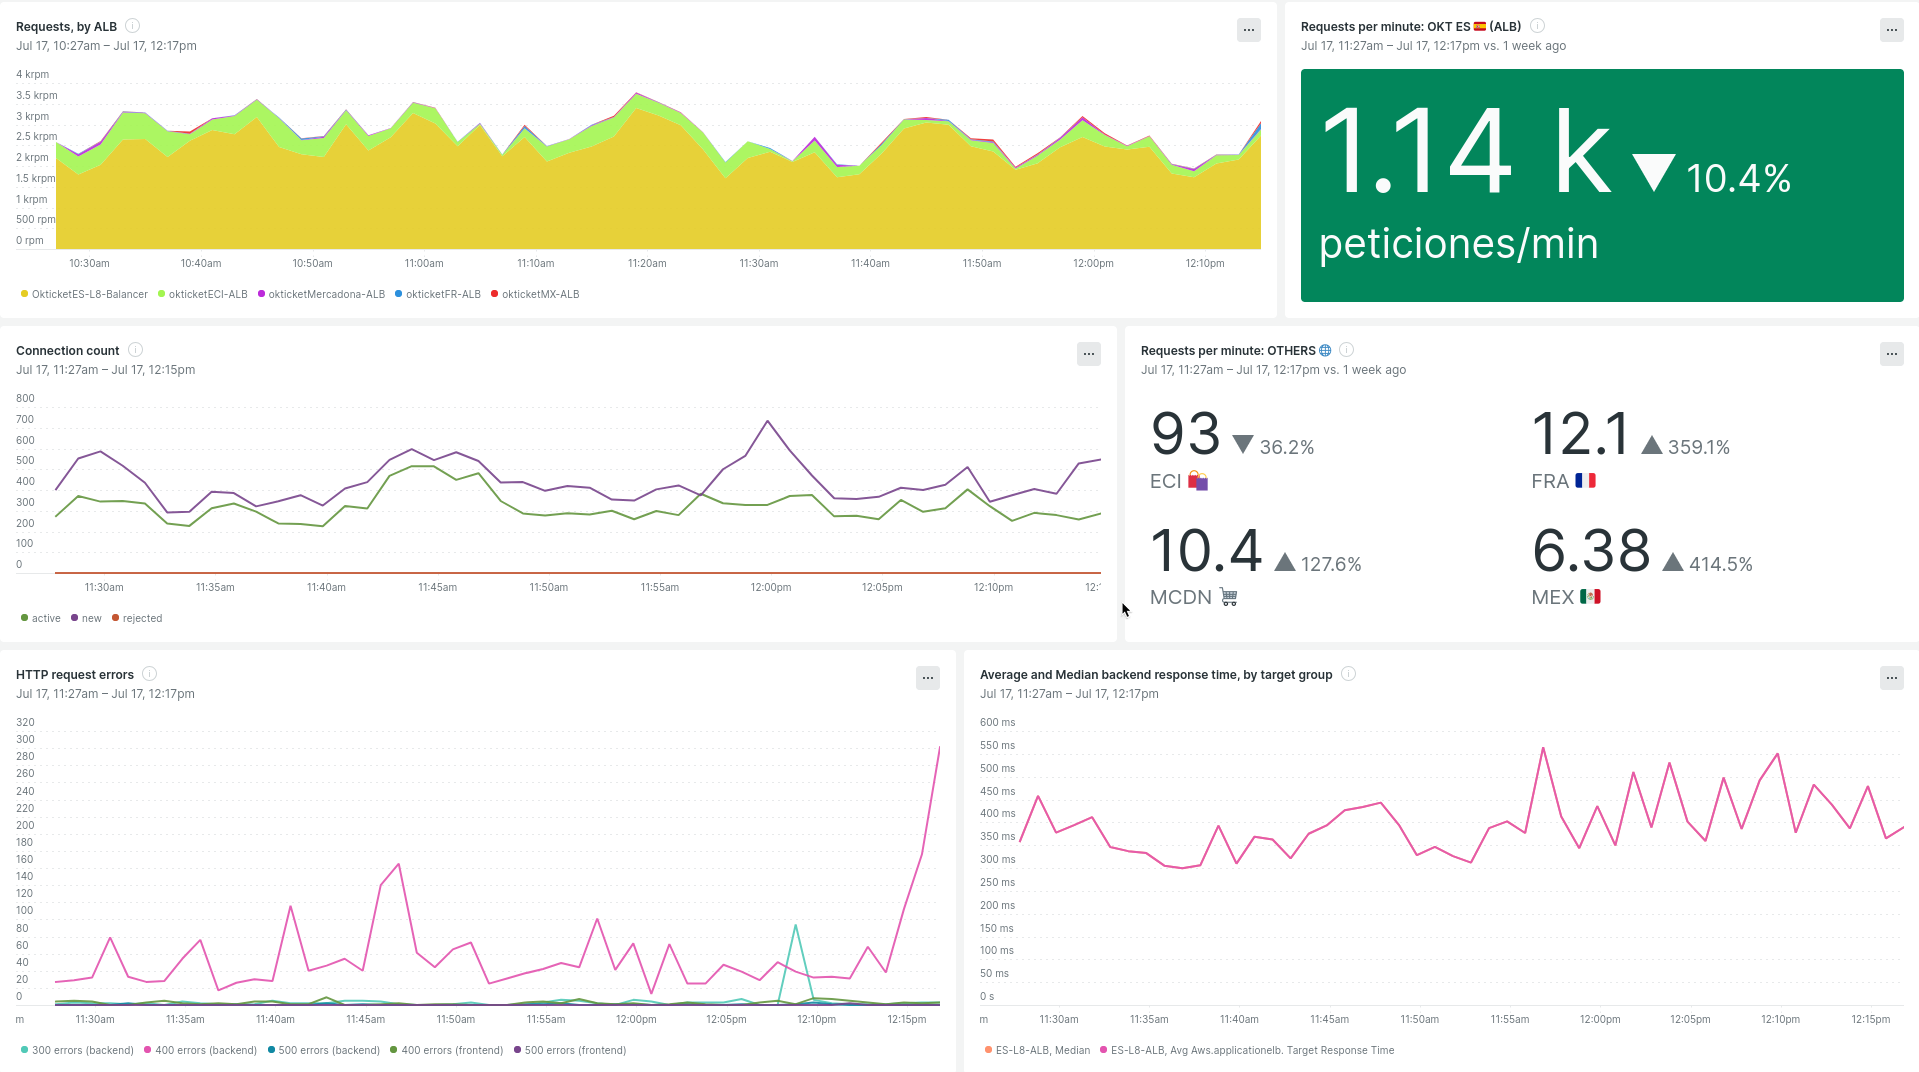
\includegraphics[width=\textwidth]{impl/dashboard_a.png}
	\caption{Dashboard de estado general de infraestructura}
	\label{fig:dashboard_a}
\end{figure}

\begin{figure}[H]
	\centering
	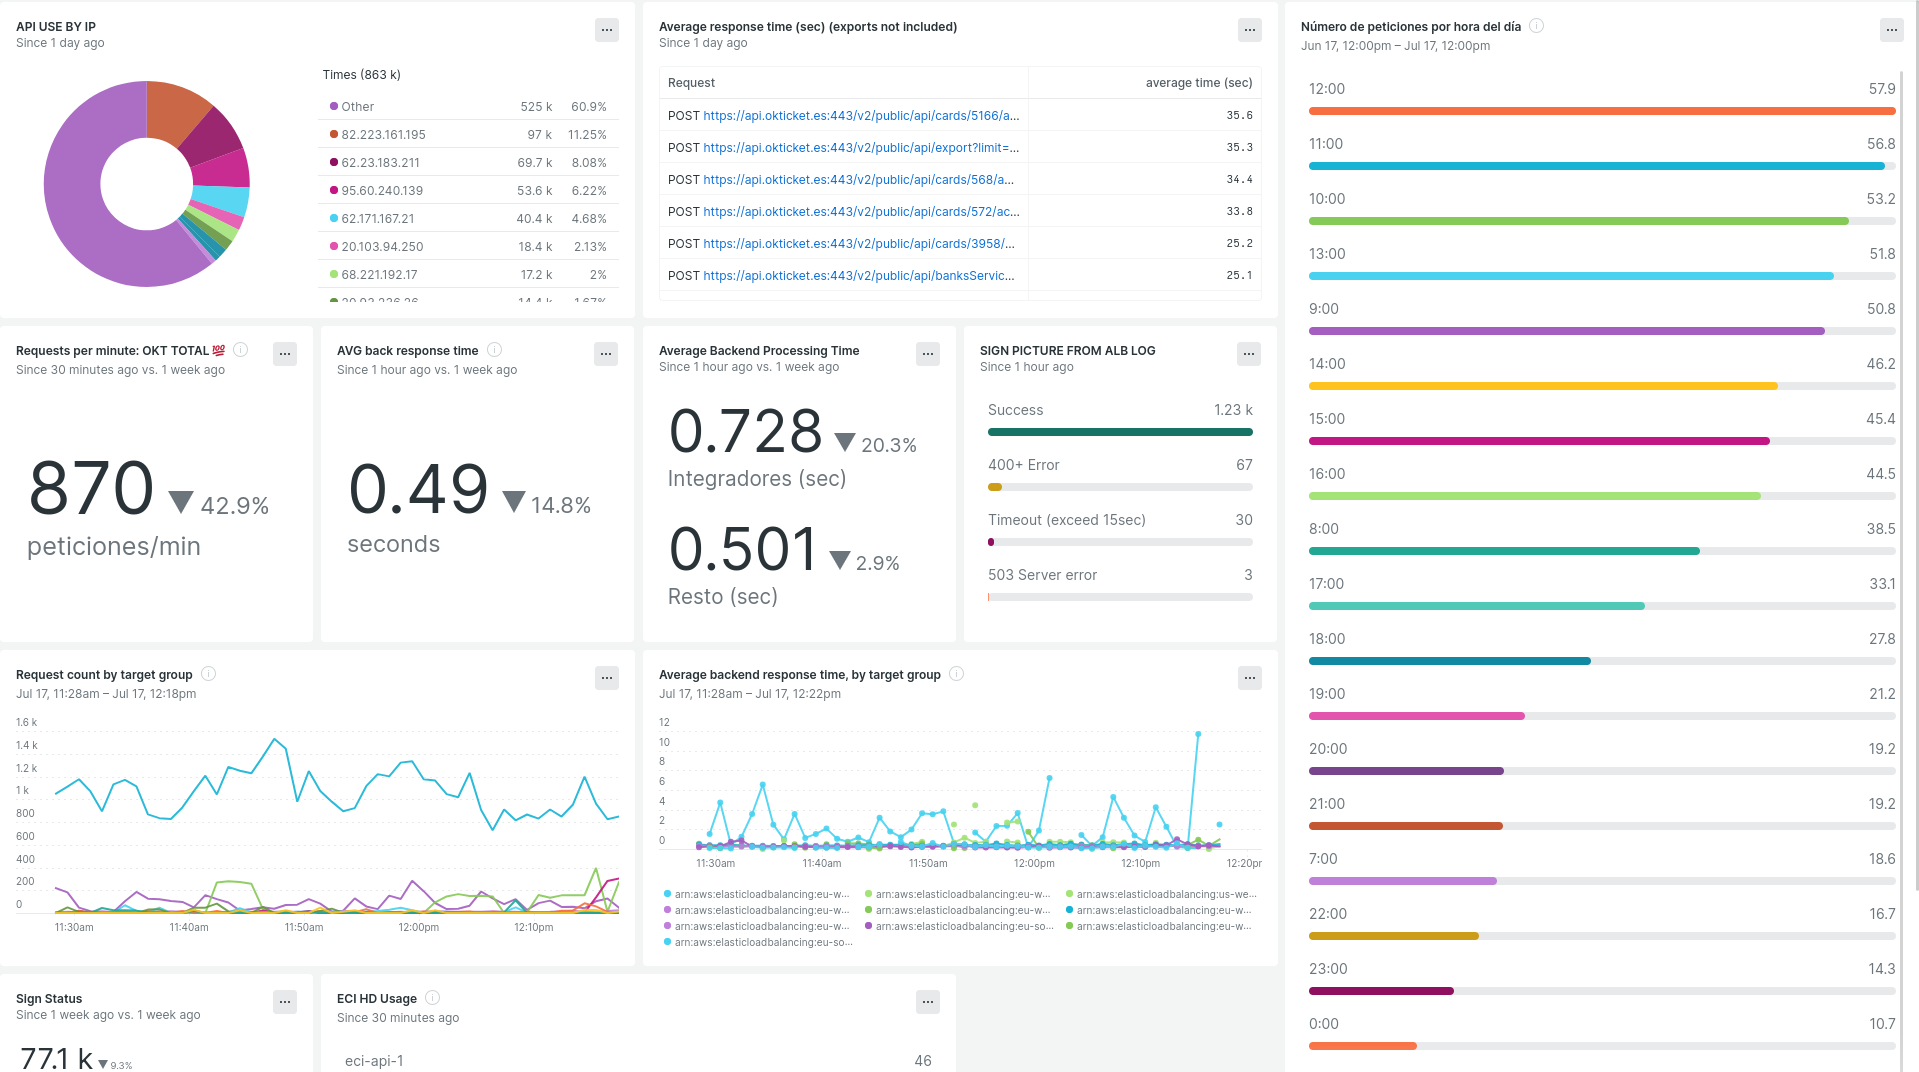
\includegraphics[width=\textwidth]{impl/dashboard_b.png}
	\caption{Dashboard de métricas detalladas}
	\label{fig:dashboard_b}
\end{figure}

